\documentclass[twoside,12pt]{report}
\usepackage[T1]{fontenc}
\usepackage[utf8]{inputenc}
\usepackage[magyar]{babel}
\usepackage[margin=3cm]{geometry}
\usepackage[section]{placeins}
\usepackage{amsmath,amssymb,tikz,fancyhdr,commath,multirow,amsthm,gensymb,etoolbox,csquotes,float,outlines,mathtools,pgfplots,makecell}
\setquotestyle[quotes]{german}
\usetikzlibrary{shapes,decorations.pathreplacing,arrows,fit}

\title{Tételek: Matematika}
\author{Horváth Dávid}
\graphicspath{{Figures/}}
\newcommand\getcurrentref[1]{%
	\ifnumequal{\value{#1}}{0}
	{Tartalomjegyzék}
	{\the\value{#1}. tétel}%
}
\newcommand\addvmargin[1]{
	\node[fit=(current bounding box),inner ysep=#1,inner xsep=0]{};
}
\fancyhead[LE,RO]{\getcurrentref{chapter}}
\fancyhead[RE,LO]{Horváth Dávid}
\newtheorem{theorem}{Tétel}[section]
\theoremstyle{definition}
\newtheorem{definition}[theorem]{Definíció}
\newtheorem{claim}{Állítás}[theorem]
\linespread{1.3}
\setlength{\parskip}{0em}
\begin{document}
\pagestyle{fancy}
\maketitle
\tableofcontents
\pagebreak
\chapter{Halmazok}
\section{Halmazok, halmazműveletek}
	A halmaz és a halmaz eleme alapfogalom, ezért nem definiáljuk, azonban úgy kell megadjuk, hogy mindenről egyértelműen eldönthető legyen, eleme vagy sem.
	
	A halmazokat nyomtatott nagybetűvel, a halmaz elemeit kisbetűvel jelöljük.
	
	\vspace{1 em}
	
	\noindent
	\textbf{Halmazok megadási módjai:}
	\begin{itemize}
		\item Elemek felsorolásával
			\subitem Pl.: A=\{0;2;4;6\}
		\item Elemeket egyértelműen meghatározó utasítással
			\subitem Pl.: B=\{páros számok\}
		\item Szimbólumokkal
			\subitem Pl.: A=\{$x|x^2>9$\}
		\item Venn-diagrammal
			\subitem 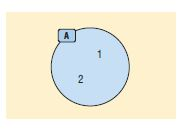
\includegraphics[]{Venn}
	\end{itemize}

	\begin{definition}
		Két halmaz egyenlő, ha ugyanazokat az elemeket tartalmazzák
	\end{definition}
	\begin{definition}
		Az elem nélküli halmazt üres halmaznak nevezzük.\\
		Jele:\{\}, vagy $\emptyset$
	\end{definition}
	\begin{definition}
		Az A halmaz részhalmaza a B halmaznak, ha A minden eleme a B halmaznak is eleme.\\
		Jele: $A\subseteq B$
	\end{definition}
	\begin{definition}
		Az A halmaz valódi részhalmaza a B halmaznak, ha A részhalmaza a B-nek, de nem
		egyenlő vele.\\
		Jele: $A\subset B$
	\end{definition}
	
	\noindent
	\textbf{Tulajdonságok:}
	\begin{itemize}
		\item $\emptyset\subseteq A$
		\item $A\subseteq A$
		\item $A\subseteq B \wedge B\subseteq A \implies A=B $
		\item $A\subseteq B \wedge B\subseteq C \implies A\subseteq C$
	\end{itemize}
	\begin{theorem}
		Az $n$ elemű halmaz összes részhalmazainak száma $2^n$.
	\end{theorem}
	\begin{proof}
		Az n elemű halmaznak $\binom{n}{k}$ darab k elemű részhalmaza van, mert így tudunk n elemből k elemet kiválasztani. Így az összes részhalmazok száma:
		\begin{equation}
			\sum_{k=0}^{n}\binom{n}{k}\label{eq:1}
		\end{equation}	
		A binomiális tétel miatt:
		\begin{equation}
			2^n=(1+1)^n=\sum_{k=0}^{n}\binom{n}{k}*1^k*1^{n-k}=\sum_{k=0}^n \binom{n}{k}\label{eq:2}
		\end{equation}
		Mivel \eqref{eq:1}=\eqref{eq:2}, ezért a részhalmazok száma $2^n$.
	\end{proof}
\section{Halmazműveletek}
	\begin{definition}
		Azt a halmazt, amelynek a vizsgált halmazok részhalmazai, alaphalmaznak vagy
		univerzumnak nevezzük.\\
		Jele: $U$ vagy $H$.
	\end{definition}
	\begin{definition}
		Egy A halmaz komplementer halmazának az alaphalmaz azon elemeinek halmazát
		nevezzük, amelyek az A halmaznak nem elemei.\\
		Jele: $\overline{A}$
	\end{definition}
	\begin{definition}
		Két vagy több halmaz uniója azon elemek halmaza, amelyek legalább az egyik halmaznak elemei.\\
		Jele: $\cup$
	\end{definition}
	\begin{definition}
		Két vagy több halmaz metszete azoknak az elemeknek a halmaza, amelyek mindegyik halmaznak elemei.\\
		Jele: $\cap$
	\end{definition}
	\begin{definition}
		A és B halmaz diszjunkt, ha $A\cap B=\emptyset$
	\end{definition}
	\begin{definition}
		Az A és B halmaz különbsége az A halmaz azon elemeinek halmaza, amelyek a B halmaznak nem elemei.\\
		Jele: $A\setminus B$
	\end{definition}
	\begin{definition}
		Az A és B halmaz szimmetrikus differenciája azon elemek halmaza, melyek csak az egyik halmaznak elemei.\\
		Jele: $A\ \Delta\ B=(A\setminus B)\cup(B\setminus A)=(A\cup B)\setminus(A\cap B)$
	\end{definition}
	\begin{definition}
		Az A és B halmaz Descartes-féle szorzata az a halmaz, amelynek elemei az összes
		olyan rendezett $(a; b)$ pár, amelynél $a\in A$ és $b\in B$.\\
		Jele: $A \times B$
	\end{definition}
	\noindent
	\subsection{Tulajdonságok:}
		\begin{itemize}
			\item Komplementer
				\begin{equation*}
					\overline{\overline{A}}=A
				\end{equation*}
			\item Unió
				\begin{align*}
					A\cup\emptyset&=A\\
					A\cup A&=A\\
					A\cup\overline{A}&=U\\
					A\cup U&=U\\
					A\cup B&=B\cup A\tag{Kommutatív}\\
					(A\cup B)\cup C&=A\cup(B\cup C)\tag{Asszociatív}\\
					A\cup(B\cap C)&=(A\cup B)\cap(A\cup C)\tag{Metszetre nézve disztributív}
				\end{align*}
			\item Metszet
				\begin{align*}
					A\cap\emptyset&=\emptyset\\
					A\cap A&=A\\
					A\cap \overline{A}&=\emptyset\\
					A\cap U&=A\\
					A\cap B&=B\cap A\tag{Kommutatív}\\
					(A\cap B)\cap C&=A\cap(B\cap C)\tag{Asszociatív}\\
					A\cap(B\cup C)&=(A\cap B)\cup(A\cap C)\tag{Unióra nézve disztributív}
				\end{align*}
			\item De-Morgan azonosságok
				\begin{align*}
					\overline{A\cup B}&=\overline{A}\cap\overline{B}
				\end{align*}
		\end{itemize}
\section{Nevezetes ponthalmazok a síkban és a térben}
	\begin{definition}
		Azoknak a pontoknak a halmaza a síkon, amelyek a sík egy adott O pontjától adott
		r távolságra vannak, egy O középpontú, r sugarú kör.
	\end{definition}
	\begin{definition}
		Azoknak a pontoknak a halmaza a térben, amelyek a tér adott O pontjától adott r távolságra
		vannak, egy O középpontú, r sugarú gömb.
	\end{definition}
	\begin{definition}
		Adott egyenestől adott távolságra lévő pontok halmaza a síkon az egyenessel párhuzamos
		egyenespár.
	\end{definition}
	\begin{definition}
		Adott egyenestől adott távolságra lévő pontok halmaza a térben olyan hengerfelület,
		amelynek tengelye az adott egyenes.
	\end{definition}
	\begin{definition}
		Két ponttól egyenlő távolságra lévő pontok halmaza a síkban a két pontot összekötő szakasz felezőmerőleges	egyenese.
	\end{definition}
	\begin{definition}
		Két ponttól egyenlő távolságra lévő pontok halmaza a térben a két pontot összekötő szakasz felezőmerőleges síkja.
	\end{definition}
	\begin{definition}
		A középpárhuzamos a síkban két párhuzamos egyenestől egyenlő távolságra lévő pontok halmaza. Olyan egyenes, amely a két adott egyenessel párhuzamos és távolságukat felezi.
	\end{definition}
	\begin{definition}
		Két metsző egyenestől egyenlő távolságra lévő pontok halmaza az általuk bezárt szögek
		szögfelező egyenesei. Két ilyen egyenes van, ezek merőlegesek egymásra.
	\end{definition}
	\begin{definition}
		Egy egyenestől és egy rajta kívül lévő ponttól egyenlő távolságra lévő pontok halmaza
		a síkon a parabola.
	\end{definition}
	Az adott pont a parabola fókuszpontja, az adott egyenes a parabola vezéregyenese (direktrixe),
	a pont és az egyenes távolsága a parabola paramétere.
\section{Egyéb ponthalmazok}
	\begin{definition}
		Azoknak a pontoknak a halmaza a síkon, amelyeknek a sík két különböző adott pontjától
		mért távolságösszege az adott pontok távolságánál nagyobb állandó: ellipszis.
	\end{definition}
	A két adott pont az ellipszis fókuszpontjai, az őket összekötő szakasz az ellipszis nagytengelye. A nagytengely felezőmerőlegesének ellipszisen belüli része az ellipszis kistengelye
	\begin{definition}
		Azoknak a pontoknak a halmaza a síkon, amelyeknek a sík két különbözõ adott pontjától
		mért távolságkülönbségének abszolút értéke a két adott pont távolságánál kisebb állandó:
		hiperbola.
	\end{definition}
	A két pont a hiperbola fókuszpontjai, az őket összekötő szakasz, a hiperbola főtengelye.
	\begin{theorem}
		Három adott ponttól egyenlő távolságra lévő pontok halmaza a síkon egy pont, ha a 3 pont
		nem esik egy egyenesre, vagy üres halmaz, ha a 3 pont egy egyenesre esik.
	\end{theorem}
	\begin{theorem}
		A háromszög három oldalfelező merőlegese egy pontban metszi egymást.
	\end{theorem}
	\begin{theorem}
	A háromszög oldalfelező merőlegeseinek metszéspontja a háromszög köré írt kör középpontja.	Ez a pont hegyesszögű háromszögnél a háromszögön belül, derékszögűnél az átfogó felezőpontjában, míg tompaszögűnél a háromszögön kívül található.
	\end{theorem}
	\begin{theorem}
		Három adott ponttól egyenlõ távolságra lévõ pontok halmaza a térben egy olyan egyenes,
		amely áthalad a három pont, mint háromszög köré írható kör középpontján, és merõleges
		a 3 pont síkjára, ha a 3 pont nem esik egy egyenesbe, vagy üres halmaz, ha a 3 pont egy
		egyenesbe esik.
	\end{theorem}
	\pagebreak
	\begin{theorem}
		Három egyenstől egyenlő távolságra lévő pontok halmaza a síkon:
		\begin{itemize}
			\item Üres halmaz, ha a három egyenes párhuzamos.
			\item Ha 2 egyenes párhuzamos, egy pedig metszi õket, akkor a 2 párhuzamos egyenes középpárhuzamosán két olyan pont, amelyek illeszkednek két metszõ egyenes szögfelezőire.
			\item Ha a 3 egyenes 3 különbözõ pontban metszi egymást, akkor szögfelezõ egyeneseik metszéspontjai. 4 ilyen pont van, az egyik a háromszög beírt körének, 3 pedig a háromszög hozzáírt köreinek középpontja.
			\item Ha a 3 egyenes egy pontban metszi egymást, akkor egyetlen pont, a 3 egyenes metszéspontja.
		\end{itemize}
	\end{theorem}
	\begin{definition}
		A látókörívek azon pontoknak a halmaza a síkon, amelyekből egy adott szakasz adott a szögben ($0\degree < \alpha < 180\degree$) látszik. Két, a szakasz egyenesére szimmetrikusan elhelyezkedő körív.
	\end{definition}
\section{Alkalmazások}
	\begin{itemize}
		\item A függvényekkel kapcsolatban is használjuk a halmazokat (értelmezési tartomány, értékkészlet).
		\item Egyenletek értelmezési tartományának vizsgálatakor számhalmazok metszetét képezzük.
		\item Koordináta-geometriában a kör, a parabola, az ellipszis és a hiperbola egyenletének felírásakor az adott görbe definícióját használjuk fel.
	\end{itemize}
\chapter{Racionális és irracionális számok}
\section{Számhalmazok}
	\begin{definition}
		A természetes számok halmaza ($\mathbb{N}$) a pozitív egész számokból és a 0-ból áll.
		
		Zárt az összeadásra, és a szorzásra nézve, azonban a kivonásra és az osztásra nem. Pl.:
		\begin{equation*}
			3-x=5
		\end{equation*}
	\end{definition}
	\begin{definition}
		Az egész számok halmaza ($\mathbb{Z}$) a természetes számokból és azok ellentettjeiből áll.
		
		Zárt a kivonásra nézve is, azonban az osztásra nem. Pl.:
		\begin{equation*}
			2x+3=4
		\end{equation*}
	\end{definition}
	\begin{definition}
		A racionális számok halmaza ($\mathbb{Q}$) azokból a számokból áll, amelyek felírhatók két egész szám hányadosaként, azaz $\frac{a}{b}$ alakban, ahol $a,b\in\mathbb{Z}\wedge b\ne0$.
		
		Mind a négy alapműveletre nézve zárt, de létezik egyenlet, amelynek nincs megoldása a halmazon, pl.:
		\begin{equation*}
			2x^2-3=0
		\end{equation*}
	\end{definition}
	\begin{definition}
		Azokat a számokat, amelyek nem írhatók fel két egész szám hányadosaként, irracionális
		számoknak ($\mathbb{Q}$*) nevezzük.
		
		Az irracionális számok halmaza nem zárt a négy alapműveletre, tizedes tört alakjuk végtelen nem szakaszos tizedes tört.
	\end{definition}
	\begin{definition}
		A racionális és az irracionális számok halmaza diszjunkt halmazok, uniójuk a valós számok halmaza($\mathbb{R}$).
		
		A valós számok halmaza zárt a négy alapműveletre.
	\end{definition}
	\begin{theorem}
		$\sqrt{2}$ irracionális szám.
	\end{theorem}
	\begin{proof}
		A bizonyítás indirekt módon történik. Tegyük fel, hogy 
		\begin{equation}\label{eq:2.1}
		\sqrt{2}=\frac{a}{b}\qquad a\wedge b\in\mathbb{Z}\wedge b\ne0\wedge(a;b)=1
		\end{equation}
		Ebből következik, hogy:
		\begin{equation}
			2=\frac{a^2}{b^2}\implies a^2=2b^2
		\end{equation}
		Az egyenlet jobb oldalán szereplő szám prímtényezős felbontásában a 2 páros kitevőn szerepel, míg a bal oldalon levő szám prímtényezős felbontásában a 2 kitevője páratlan.
		
		Ez azonban lehetetlen, hiszen a számelmélet alaptétele szerint egy pozitív egész számnak
		nincs két lényegesen különböző felbontása. 
		
		Emiatt \eqref{eq:2.1} hamis, vagyis $\sqrt{2}$ irracionális.
	\end{proof}
\section{Műveletek a racionális számok halmazán}
	Egy közönséges tört értéke nem, csak az alakja változik, ha a számlálóját és a nevezőjét ugyanazzal a 0-tól különböző számmal szorozzuk (bővítés), vagy ugyanazzal a 0-tól különböző számmal osztjuk (egyszerűsítés).
	
	Ha a racionális számok közönséges tört alakúak, akkor a következő szabályokkal lehet elvégezni az alapműveleteket:
	\begin{itemize}
		\item Csak azonos nevezőjű törteket lehet összeadni, kivonni, ezért a törteket bővítjük egy közös többszörösű nevezőre:
		\begin{equation*}
			\frac{a}{b}\pm\frac{c}{d}=\frac{a*d}{b*d}\pm\frac{c*b}{d*b}=\frac{a*d\pm c*b}{b*d}\qquad \text{Ahol}\ b\wedge d\ne0
		\end{equation*}
		\item Törtet törttel úgy szorzunk, hogy a számlálót a számlálóval, nevezőt a nevezővel szorozzuk:
		\begin{equation*}
		\frac{a}{b}*\frac{c}{d}=\frac{a*c}{b*d}\qquad \text{Ahol}\ b\wedge d\ne0
		\end{equation*}
		\item Törtet törttel úgy osztunk, hogy a változatlan osztandót szorozzuk az osztó reciprokával:
		\begin{equation*}
		\frac{a}{b}:\frac{c}{d}=\frac{a}{b}*\frac{d}{c}=\frac{a*d}{b*c}\qquad \text{Ahol}\ b\wedge d\ne0
		\end{equation*}
	\end{itemize}
\section{Műveletek az irracionális számok halmazán}
	Az alapműveletek definiálhatók az irracionális számok körében úgy, hogy az eddigi azonosságok életben maradjanak. Mivel tizedestört alakjuk végtelen, nem periodikus, így azt csak közelítően tudjuk megadni. Ezért a pontos értékeket pl. hatvány, gyök, logaritmus alakban adjuk meg, ilyenkor	viszont a megfelelő műveleti szabályokkal dolgozunk.
\section{Műveleti tulajdonságok a valós számok halmazán}
	\begin{itemize}
		\item Az összeadás és a szorzás kommutatív
		\item Az összeadás és a szorzás asszociatív
		\item A szorzás az összeadásra nézve disztributív
	\end{itemize}
\section{Közönséges és tizedes törtek}
	Az $\frac{a}{b}$ hányados a következő alakokban fordulhat elő ($a,b\in\mathbb{Z},b\ne0, (a;b)=0$):
	\begin{itemize}
		\item Egész szám, ha $b\ \vline\ a$
		\item Véges tizedestört, ha b prímtényezõs felbontásában a 2 és az 5 számokon kívül nincs más prímszám
		\item Végtelen szakaszos tizedestört, ha b prímtényezõs felbontásában a 2 és az 5 számokon kívül	más prímszám is van.
	\end{itemize}
	A tizedestörtek formái lehetnek:
	\begin{itemize}
		\item véges tizedestörtek
		\item végtelen tizedestörtek, ezek lehetnek
			\begin{itemize}
				\item szakaszos tizedestörtek, ezek felírhatók közönséges tört alakban. Pl. végtelen mértani sor összegeként.
				\item nem szakaszos tizedestörtek, ezek nem írhatók át közönséges tört alakba
			\end{itemize}
	\end{itemize}
\section{Halmazok számossága}
	\begin{definition}
		Egy A halmaz számossága az A halmaz elemeinek számát jelenti. Jele: |A|. Egy
		halmaz számossága lehet véges vagy végtelen.
	\end{definition}
	\begin{definition}
		Egy halmaz véges halmaz, ha elemeinek számát egy természetes számmal megadhatjuk. Ellenkező esetben végtelen halmazról beszélünk. Végtelen halmazok számosságát $\aleph$-el jelöljük.
	\end{definition}
	\begin{definition}
		A pozitív természetes számokkal megegyező számosságú halmazokat megszámlálhatóan végtelen halmazoknak nevezzük. Jele:$\aleph_0$.
		
		Megszámlálhatóan végtelen számosságúak: egész számok, páros számok, négyzetszámok, racionális számok.
	\end{definition}
	\begin{theorem}
		A valós számok halmazának számossága nem egyezik meg a pozitív természetes számok halmazának számosságával.
	\end{theorem}
	\begin{proof}
		Tegyük fel, hogy a valós számok halmaza megszámlálhatóan végtelen számosságú, azaz sorba rendezhetőek. Ekkor a 0, és 1 közötti valós számok is sorba rendezhetőek. Bizonyításomban csak ezekkel a számokkal fogok foglalkozni, mivel ha nem rendezhetőek sorba, akkor a valós számok sem. Képezzünk egy számot a következő módon:
		\begin{itemize}
			\item Egészrésze 0
			\item Az első valós szám első tizedesjegyétől, a második második tizedesjegyétől, ... eggyel eltér
		\end{itemize}
		Ez a szám nem egyezik egyik sorba rendezett számmal sem, emiatt nem rendezhetőek sorba. Azaz a valós számok halmazának számossága nem egyezik meg a pozitív természetes számok halmazának számosságával.
	\end{proof}
	\begin{definition}
		A valós számok számosságával megegyező számosságú halmazokat nem megszámlálhatóan
		végtelen vagy kontinuum számosságú halmazoknak nevezzük. $\aleph_\mathbb{R}=2^{\aleph_0}$
		
		Pl.: irracionális számok halmaza, számegyenes pontjainak halmaza, intervallum pontjainak halmaza.
	\end{definition}
\section{Alkalmazások}
	\begin{itemize}
		\item Racionális számok: arányok, arányosság, hasonlóság
		\item Irracionális számok: szabályos háromszög magassága, négyzet átlója, kör kerülete, területe.
		\item Kifejezések legbővebb értelmezési tartományának meghatározása.
		\item Függvény értékkészletének megállapítása
	\end{itemize}
\chapter{Oszthatóság}
\section{Oszthatóság}
	\begin{definition}
		Egy $a$ egész szám osztója egy $b$ egész számnak, ha található olyan $c$ egész szám,
		amelyre $a*c=b$. Jelölése: $a\vert b$. Ebben az esetben az is igaz, hogy $b$ osztható $a$-val és $c$-vel. Ekkor azt is mondhatjuk, hogy $b$ többszöröse $a$-nak.
	\end{definition}
	\begin{itemize}
		\item A 0 minden nemnulla egész számnak többszöröse, azaz a 0 minden nemnulla egész számmal osztható. Ez azt is jelenti, hogy a 0 páros. A 0-nak egyetlen többszöröse van a 0.
		\item A 0 nem osztója egyetlen nemnulla egész számnak sem.
	\end{itemize}
	\begin{theorem}[Oszthatósági tételek]
		Ha $a,b,c\in\mathbb{Z}$
		\begin{itemize}
			\item $1\vert a$
			\item $a\vert a$
			\item $a\vert b\wedge b\vert c\implies a\vert c$
			\item $a\vert b\implies a\vert(b*c)$
			\item $a\vert b\wedge a\vert c\implies a\vert (b\pm c)$
			\item $a\vert b\wedge a\vert (b+c)\implies a\vert c$
		\end{itemize}
	\end{theorem}
	Az oszthatóságot eddig az egész számokra értelmeztük, a továbbiakban leszűkítjük a természetes számokra.
	\begin{theorem}
		Ha $a, b\in \mathbb{Z}^+$, $a\vert b\wedge b\vert a\implies a=b$
	\end{theorem}
	\noindent
	\subsection{Oszthatósági szabályok}
	Egy $n$ egész szám osztható
	\begin{itemize}
		\item 2-vel, ha n utolsó jegye 0,2,4,6, vagy 8.
		\item 3-mal, ha számjegyeinek összege osztható 3-mal
		\item 4-gyel, ha a két utolsó jegybõl képzett szám osztható 4-gyel.
		\item 5-tel, ha utolsó jegye 0, vagy 5.
		\item 6-tal, ha 2-vel és 3-mal osztható.
		\item 7-tel, ha $10x+y$ alakú, és $x-2y$ osztható 7-tel, ahol $x,y\in\mathbb{N}$
		\item 8-cal, ha a három utolsó jegybõl képzett szám osztható 8-cal.
		\item 9-cel, ha számjegyeinek összege osztható 9-cel.
		\item 10-zel, ha utolsó jegye 0.
	\end{itemize}
\section{Prímszám, összetett szám, számelmélet alaptétele, osztók száma}
	\begin{definition}
		Azokat a pozitív egész számokat, amelyeknek pontosan két pozitív osztója van, prímszámoknak nevezzük.
	\end{definition}
	\begin{theorem}
		Végtelen sok prímszám van.
	\end{theorem}
	\begin{proof}
		Indirekt módon: Tegyük fel, hogy n db prímszám van, az i-ediket jelölje: $p_i$. Képezzük az $A=\prod_{i=1}^{n} (p_i)+1$ számot.
		
		Ennek a felsorolt prímek egyike sem osztója. Két lehetőség van, vagy A prím, vagy létezik olyan prím, amit nem soroltunk fel. Mindkét esetben ellentmondásra jutottunk, tehát végtelen sok prímszám van.
	\end{proof}
	\begin{definition}
		Azokat az 1-nél nagyobb számokat, amelyek nem prímszámok, összetett számoknak
		nevezzük.
	\end{definition}
	\begin{theorem}[Számelmélet alaptétele]
		Bármely összetett szám felírható prímszámok szorzataként, és ez a felbontás a tényezők sorrendjétől eltekintve egyértelmű.
	\end{theorem}
	Kanonikus alak: $n=\prod_{i=1}^{k}p_i^{\alpha_i}$, ahol $p_i$ prímszám, $\alpha_i$ nemnegatív egész szám. Ekkor az n szám prímosztói: $p_1,p_2,...,p_k$.
	\begin{theorem}
		$n=\prod_{i=1}^{k}p_i^{\alpha_i}$ osztóinak száma: $\prod_{i=1}^{k}(\alpha_i+1)$
	\end{theorem}
	\begin{definition}
		Két vagy több pozitív egész szám legnagyobb közös osztója a közös osztók közül a legnagyobb. Jele: $(a; b)$.
	\end{definition}
	Előállítása: a számok prímtényezős alakjában, a közös prímtényezőket a hozzájuk tartozó legkisebb kitevővel vesszük és összeszorozzuk.
	\begin{equation*}
		\left(\prod_{i=1}^{k}p_i^{\alpha_i};\prod_{i=1}^{k}p_i^{\beta_i}\right)=
		\prod_{i=1}^{k} p_i^{\text{min}(\alpha_i,\beta_i)}
	\end{equation*}
	\begin{definition}
		Ha két pozitív egész szám legnagyobb közös osztója 1, akkor a két szám relatív prím.
	\end{definition}
	\begin{definition}
		Két vagy több pozitív egész szám legkisebb közös többszöröse a közös többszörösök
		közül a legkisebb. Jele: $[a; b]$.
	\end{definition}
	Előállítása: felírjuk a számok prímtényezős alakját, az összes prímtényezőt	a hozzájuk tartozó legnagyobb kitevővel vesszük és összeszorozzuk.
	\begin{gather*}
		\left(\prod_{i=1}^{k}p_i^{\alpha_i};\prod_{i=1}^{k}p_i^{\beta_i}\right)=
		\prod_{i=1}^{k} p_i^{\text{max}(\alpha_i,\beta_i)}\\
		(a;b)*[a;b]=a*b
	\end{gather*}
\section{Számrendszerek}
	\begin{definition}
		Az a alapú számrendszer helyi értékei: $a^k$, ahol $k\in\mathbb{N}$. Az a alapú számrendszerben a-féle számjegy van: $0,1,...,a-1$, ha a>10, betűket használunk számjegyként.
	\end{definition}
	A helyi értékes ábrázolás azt jelenti, hogy a számjegyek értékén kívül a leírásuk helye is értékkel bír. Általában 10-es számrendszerben dolgozunk, a helyi értékek 10 természetes kitevőjű hatványai, a számok leírására 10 számjegyre van szükség. Az informatikában gyakran használják a 2-es, vagyis bináris, és a 16-os, azaz hexadecimális számrendszert.
	\subsection{Áttérés 10-es számrendszerből más alapúba}
	A számot osztjuk az új számrendszer alapszámával, majd az így kapott hányadost újra mindaddig, míg 0 hányadost nem kapunk. Az osztásoknál kapott maradékok lesznek az új szám alaki értékei az egyesektől kezdve.
	\subsection{Áttérés más alapúból 10-es számrendszerbe}
	A megfelelő helyi értékeknek és a hozzájuk tartozó alaki értékeknek a szorzatösszege adja a 10-es számrendszerbeli értéket.
\section{Alkalmazások}
	\begin{itemize}
		\item Legnagyobb közös osztó: törtek egyszerűsítése
		\item Legkisebb közös többszörös: törtek közös nevezőre hozása
		\item Kétismeretlenes egyenlet megoldása a természetes számok halmazán
	\end{itemize}
\chapter{Logika}
\section{A matematikai logika fogalma}
	A matematikai logika a gondolkodás matematikai formában kifejezhető, matematikai eszközökkel	vizsgálható összefüggéseinek, törvényeinek feltárásával foglalkozik. Fõ feladata a következtetések helyességének vizsgálata.
\section{Logikai műveletek}
	\begin{definition}[Állítás]
		Olyan kijelentő mondat, amelyről egyértelműen el lehet dönteni, hogy igaz vagy hamis.
	\end{definition}
	\begin{definition}
		Az igaz és a hamis a kijelentés logikai értéke.
	\end{definition}
	Ha az A állítás igaz, a B állítás hamis, akkor $|A|=i$ és $|B|=h$. Az igaz értéket szokták 1-gyel, a hamisat 0-val jelölni.
	\begin{definition}
		A kijelentéseket összekapcsolhatjuk. Azokat a kijelentéseket, amelyeket más kijelentésekből lehet előállítani, összetett kijelentéseknek nevezzük.
	\end{definition}
	\begin{definition}
		Ha az összetett kijelentések logikai értéke csak az õt alkotó állítások logikai értékétől és az előállítás módjától függ, akkor logikai műveletekről beszélünk.
	\end{definition}
	Logikai műveleteket igazságtábla segítségével végezhetünk el.
	\begin{definition}
		Az állítás tagadása egyváltozós művelet. Egy A kijelentés negációja	az a kijelentés, amely akkor igaz, ha A hamis és akkor hamis, ha A igaz. Jele: $\overline{A}$  vagy $\neg A$.
	\end{definition}
	\begin{theorem}[Kettős tagadás törvénye]
		Egy állítás tagadásának tagadása az állítás: $\neg\neg A=A$.
	\end{theorem}
	\begin{theorem}[Ellentmondásmentesség elve]
		Egy állítás és tagadása nem lehet egyszerre igaz.
	\end{theorem}
	\begin{theorem}[A harmadik kizárásának elve]
		Egy állítás és tagadása nem lehet egyszerre hamis.
	\end{theorem}
	\begin{definition}
		Két, A-tól és B-tõl függő állítás akkor egyenlő, ha A és B minden lehetséges logikai
		értékére a két állítás igazságértéke egyenlő.
	\end{definition}
	\begin{definition}[Diszjunkció (megengedő vagy)]
		Két kijelentés diszjunkciója pontosan akkor igaz, ha legalább az egyik kijelentés igaz, különben hamis. Jele: $A \vee B$.
	\end{definition}
	\begin{definition}[Antivalencia (kizáró vagy)]
		Két kijelentés antivalenciája pontosan akkor igaz, ha pontosan az egyik kijelentés igaz, különben hamis. Jele: $A\oplus B$.
	\end{definition}
	\begin{definition}[Konjunkció (és)]
		Két kijelentés konjunkciója pontosan akkor igaz, ha mindkét kijelentés igaz, különben hamis. Jele: $A\wedge B$.
	\end{definition}
	\begin{definition}[Implikáció (következtetés)]
		A \enquote{ha A, akkor B} kapcsolatnak megfelelő logikai művelet. Logikai értéke pontosan akkor hamis, ha A igaz és B hamis, különben igaz. Az A állítást feltételnek, B-t következménynek nevezzük. Jele: $A\rightarrow B$
	\end{definition}
	\begin{definition}[Ekvivalencia]
		Az \enquote{A akkor és csak akkor B} kapcsolatnak megfelelő logikai művelet. Logikai értéke pontosan akkor igaz, ha A és B logikai értéke azonos, különben hamis. Jele: $A\leftrightarrow B$
	\end{definition}
	Ha $A\leftrightarrow B$ igaz, akkor A és B állítások ekvivalensek egymással.
	\subsection{Műveleti tulajdonságok}
	\begin{itemize}
		\item Diszjunkció
			\begin{align*}
				A\vee A&=A\\
				A\vee \neg A&=i\\
				A\vee B&=B\vee A\tag{Kommutatív}\\
				(A\vee B)\vee C&=A\vee(B\vee C)\tag{Asszociatív}\\
				A\vee(B\wedge C)&=(A\vee B)\wedge(A\vee C)\tag{Konjunkcióra nézve disztributív}
			\end{align*}
		\item Konjunkció
			\begin{align*}
				A\wedge A&=A\\
				A\wedge \neg A&=h\\
				A\wedge B&=B\wedge A\tag{Kommutatív}\\
				(A\wedge B)\wedge C&=A\wedge(B\wedge C)\tag{Asszociatív}\\
				A\wedge(B\vee C)&=(A\wedge B)\vee(A\wedge C)\tag{Diszjunkcióra nézve disztributív}
			\end{align*}
	\end{itemize}
	\begin{theorem}
		Tetszőleges A és B kijelentésektre $A\rightarrow B=\neg A\vee B$.
	\end{theorem}
	\begin{proof}
		Igazságtáblázattal:
		\begin{table}[H]
			\begin{tabular}{|c|c|c|c|c|c|}
				\hline
				A&B&$A\rightarrow B$&$B\rightarrow A$&$(A\rightarrow B)\wedge(B\rightarrow A)$&$A\leftrightarrow B$\\\hline
				i&i&i&i&i&i\\\hline
				i&h&h&i&h&h\\\hline
				h&i&i&h&h&h\\\hline
				h&h&i&i&i&i\\\hline
			\end{tabular}
		\end{table}
		Az ötödik oszlop igazságértékei megegyeznek az ekvivalencia igazságértékeivel, tehát az
		egyenlőség A és B minden lehetséges logikai értékére fennáll, azaz azonosság.
	\end{proof}
\pagebreak
\section{Állítás és megfordítása, szükséges és elégséges feltétel}
	\begin{outline}
		\1 $A\rightarrow B=i$
			\2 A állítás B-nek elégséges feltétele
			\2 B állítás A-nak szükséges feltétele
			\2 Ha A igazságáról B igazságára következtetünk: helyes következtetés
		\1 $A\rightarrow B=h$
			\2 Elég egy példa A=h, B=i
			\2 Ha A igazságáról B igazságára következtetünk: helytelen következtetés
		\1 $A\rightarrow B=i \wedge B\rightarrow A=i$
			\2 A állítás B-nek szükséges és elégséges feltétele
			\2 $A\Leftrightarrow B$
			\2 A és B ekvivalensek
		\1 Feltételek, következmények megcserélése: állítás megfordítása ($B\rightarrow A$)
			\2 Állítás, és megfordítása igaz: két állítás ekvivalens
				\3 Pl.: Thalész-tétel, Pitagorasz tétel
	\end{outline}
	\begin{theorem}[Thalész-tétel]
		Ha egy kör átmérőjének két végpontját összekötjük a kör bármely más
		pontjával, akkor derékszögű háromszöget kapunk.
	\end{theorem}
	\begin{theorem}[Thalész-tétel megfordítása]
		Ha egy háromszög derékszögű, akkor köré írható körének középpontja az átfogó felezőpontja.
	\end{theorem}
	\begin{theorem}[Pithagorasz-tétel]
		Ha egy háromszög derékszögű, akkor a befogók négyzetének összege egyenlő az átfogó négyzetével.
	\end{theorem}
	\begin{theorem}[Pithagorasz-tétel megfordítása]
		ha egy háromszög két oldalhosszának négyzetének összege egyenlő a harmadik oldal négyzetével, akkor a háromszög derékszögű.
	\end{theorem}
\section{Alkalmazások}
	\begin{itemize}
		\item Matematikai definíciók, tételek pontos kimondása, tételek bizonyítása
		\item Bizonyítási módszerek kidolgozása (direkt, indirekt, skatulya elv, teljes indukció)
		\item Kombinatorika, valószínűségszámítás használja a logikai műveleteket és azok tulajdonságait.
		\item Egyenletek, egyenlőtlenségek megoldása során sokszor végzünk logikai műveleteket (ekvivalens átalakítások).
	\end{itemize}
\chapter{Hatványozás, gyökvonás}
\section{Pozitív egész kitevőjű hatványok}
	\begin{definition}
		Ha $a$ tetszőleges valós szám és $n$ 1-nél nagyobb természetes szám, akkor $a^n$ hatvány
		azt az n tényezős szorzatot jelenti, amelynek minden tényezője a. Ha n=1, $a^1=a$.
	\end{definition}
	Az $a$ számot a hatvány alapjának, az $n$ számot a hatvány kitevőjének nevezzük.
	\begin{theorem}
		Azonos alapú hatványokat úgy is szorozhatunk, hogy a közös alapot a kitevők összegére
		emeljük: 
		\begin{equation*}
			a^m*a^n=a^{m+n}
		\end{equation*}
	\end{theorem}
	\begin{theorem}
		Azonos alapú hatványokat úgy is oszthatunk, hogy a közös alapot a kitevők különbségére
		emeljük: 
		\begin{equation*}
			\frac{a^m}{a^n}=a^{m-n}\text{, ha } a\ne0, m>n
		\end{equation*}.
	\end{theorem}
	\begin{theorem}
		Szorzatot tényezőnként is hatványozhatunk: 
		\begin{equation*}
			(a*b)^n=a^n*b^n
		\end{equation*}
	\end{theorem}
	\begin{theorem}
		Azonos kitevő hatványokat úgy is szorozhatunk, hogy az alapok szorzatát a közös kitevőre emeljük.
	\end{theorem}
	\begin{theorem}
		Törtet úgy is hatványozhatunk, hogy a számlálót és a nevezőt külön-külön hatványozzuk
		és a kapott hatványoknak a kívánt sorrendben a hányadosát vesszük. 
		\begin{equation*}
			\left(\frac{a}{b}\right)^n=\frac{a^n}{b^n}\text{, ha }b\ne0
		\end{equation*}
	\end{theorem}
	\begin{theorem}
		Azonos kitevőjű hatványokat úgy is oszthatunk, hogy az alapok hányadosát a közös kitevőre emeljük.
	\end{theorem}
	\begin{theorem}
		Hatványt úgy is hatványozhatunk, hogy az alapot a kitevõk szorzatára emeljük:
		\begin{equation*}
			\left(a^n\right)^m=a^{n*m}
		\end{equation*}
	\end{theorem}
\section{A hatványozás kiterjesztése}
	\begin{definition}[Permanencia-elv]
		A hatványozás fogalmát úgy terjesztjük ki, hogy az eddigi azonosságok továbbra is teljesüljenek.
	\end{definition}
	\begin{definition}
		Tetszőleges $a\ne0$ valós számra $a^0=1$.
	\end{definition}
	$0^0$-t nem értelmezzük, mert:
	\begin{itemize}
		\item 0 kéne, hogy legyen, mivel 0 minden pozitív egész kitevő hatványa 0
		\item 1 kéne, hogy legyen, mivel minden egyéb szám nulladik hatványa 1
	\end{itemize}
	\begin{definition}
		Tetszőleges $a\ne0$ valós szám és $n$ pozitív egész szám esetén $a^{-n}=\frac{1}{a^n}$
	\end{definition}
	\begin{definition}
		Az $a$ pozitív valós szám $\frac{p}{q}$-adik hatványa az a pozitív valós szám, amelynek q-adik hatványa $a^p$, azaz $\left(a^{\frac{p}{q}}\right)^q=a^p$.
	\end{definition}
	Ebből következik, hogy $a^\frac{p}{q}=\sqrt[q]{a^p}$
	\begin{definition}
		Az $a$ pozitív valós szám $\alpha$ irracionális kitevőjű hatványa, $a^\alpha$ a következő határérték: $\lim\limits_{n\rightarrow\infty} a^{r_n}$, ahol {$r_n$} egy olyan számsorozat, mely racionális számokból áll, és $\lim\limits_{n\rightarrow\infty}r_n=\alpha$.
	\end{definition}
\section{Az n-edik gyök fogalma}
	\begin{definition}
		Egy $a$ valós szám $(2k+1)$-edik $(k\in\mathbb{N}^+)$ gyökén azt a valós számot értjük, amelynek $(2k + 1)$-edik hatványa $a$. 
		\begin{equation*}
		\left(\sqrt[2k+1]{a}\right)^{2k+1}=a\text{, ahol }k\in\mathbb{N}^+
		\end{equation*}
	\end{definition}
	\begin{definition}
		Egy nemnegatív $a$ valós szám $2k$-adik $(k\in\mathbb{N}^+)$ gyökén azt a nemnegatív valós számot értjük, amelynek $2k$-adik hatványa $a$.
		\begin{equation*}
			\left(\sqrt[k]{a}\right)^k=a\text{, ahol } a\ge0,\ \sqrt[2k]{a}\ge0,\ k\in\mathbb{Z}^+
		\end{equation*}
	\end{definition}
	\begin{definition}
		Egy nemnegatív valós $a$ szám négyzetgyökén azt a nemnegatív valós számot értjük,
		amelynek négyzete $a$.
		\begin{equation*}
			\left(\sqrt{a}\right)^2=a\text{, ahol } a\ge0,\ \sqrt{a}\ge0
		\end{equation*}
	\end{definition}
	A definíciókból következően:
	\begin{equation*}
		\sqrt[n]{a^n}=
		\begin{cases}
			|a|, & \text{ha $n$ páros}\\
			a, & \text{ha $n$ páratlan}
		\end{cases}
	\end{equation*}
\section{A négyzetgyök azonosságai}
	\begin{theorem}
		$\sqrt{a*b}=\sqrt{a}*\sqrt{b}$, ha a,b nemnegatív valós számok. Szorzat négyzetgyöke egyenlő a tényezők négyzetgyökének szorzatával. Tehát szorzatból tényezőnként vonhatunk gyököt.
	\end{theorem}
	\begin{proof}
		Vizsgáljuk mindkét oldal négyzetét:
		\begin{align*}
			\left(\sqrt{a*b}\right)^2&=a*b\\
			\left(\sqrt{a}*\sqrt{b}\right)^2=\left(\sqrt{a}\right)^2*\left(\sqrt{b}\right)^2&=a*b
		\end{align*}
		Ha mindkét oldal értelmes, vagyis $a,b$ nemnegatív, akkor a két oldal négyzetének egyenlőségéből következik a két oldal egyenlősége, mivel $a*b\ge 0\text{, ha } a\ge0\wedge b\ge0$
	\end{proof}
	\begin{theorem}
		$\sqrt{\frac{a}{b}}=\frac{\sqrt{a}}{\sqrt{b}}$, ha a, b nemnegatív valós számok, $b\ne0$. Tört négyzetgyöke egyenlő a számláló és a nevező négyzetgyökének hányadosával.
	\end{theorem}
	\begin{theorem}
		$\sqrt{a^k}=\left(\sqrt{a}\right)^k$, ha $k$ egész, $a>0$ valós szám. A hatványozás és a gyökvonás sorrendje felcserélhető egymással pozitív alap esetén.
	\end{theorem}
\section{Hatványfüggvények és azok tulajdonságai}
	\begin{definition}[Hatványfüggvény]
		Az $f:\mathbb{R}\longrightarrow\mathbb{R},\ f(x)=x^n$ függvényt, ahol $n\in\mathbb{N}^+$, hatványfüggvénynek nevezzük. Értelmezhető az $n=0$ esetre is, de ettől most eltekintünk.
	\end{definition}
	\noindent
	\begin{table}[H]
		\centering
		\begin{tabular}{|m{4cm}||>{\centering\arraybackslash} m{5cm}|>{\centering\arraybackslash} m{5cm}|}
			\hline
			Kitevő&Páros&Páratlan\\\hline
			Ábrázolás&\begin{tikzpicture}[baseline=70]
			\begin{axis}[axis y line=center,
			axis x line=middle,width=6cm,ticks=none]
			\addplot+[mark=none] {x*x};
			\addvmargin{1mm}
			\end{axis}
			\end{tikzpicture}&
			\begin{tikzpicture}[baseline=70]
			\begin{axis}[axis y line=center,
			axis x line=middle,width=6cm,ticks=none]
			\addplot+[mark=none] {x*x*x};
			\end{axis}
			\addvmargin{1mm}
			\end{tikzpicture}\\\hline
			Értelmezési tartománya&$\mathbb{R}$&$\mathbb{R}$\\\hline
			Értékkészlete&$\mathbb{R}^+\cup\{0\}$&$\mathbb{R}$\\\hline
			Montonitása&ha $x<0$, szigorúan monoton csökken, ha $x>0$, szigorúan monoton nő&szigorúan monoton nő\\\hline
			Szélsőértéke&abszolút minimum: hely: $x=0$, érték: $f(x)=0$&nincs\\\hline
			Görbülete&konvex&ha $x<0$, akkor konkáv, ha $x>0$, akkor konvex\\\hline
			Zérushelye&x=0&x=0\\\hline
			Paritása&páros&páratlan\\\hline
			Korlátosság&alulról korlátos&nem korlátos\\\hline
			Invertálhatóság&\makecell{invertálható, ha $x\ge0$, \\ $f^{-1}:\left(\mathbb{R}^+\cup\{0\}\right)\longrightarrow\mathbb{R},$\\
				$\ f^{-1}(x)=\sqrt[n]{x}$} &\makecell{invertálható, \\ $f^{-1}:\left(\mathbb{R}^+\cup\{0\}\right)\longrightarrow\mathbb{R},$\\
				$\ f^{-1}(x)=\sqrt[n]{x}$}\\\hline
		\end{tabular}
	\end{table}
	Ha n=1, akkor a függvény nem konvex, és nem konkáv. Folytonosak, minden pontban differenciálhatóak, minden korlátos intervallumon integrálhatóak.
\section{Négyzetgyökfüggvény és tulajdonságai}
	\begin{definition}
		Az $f:\left(\mathbb{R}^+\cup{0}\right)\longrightarrow\mathbb{R},\ f(x)=\sqrt{x}$ függvényt négyzetgyökfüggvénynek nevezzük.
	\end{definition}
	\begin{outline}
		\1 Jellemzés
			\2 \begin{tikzpicture}[baseline=70]
			\begin{axis}[axis y line=center,
			axis x line=middle,width=10cm,ticks=none,domain=0:10,samples=1000]
			\addplot+[mark=none] {sqrt(x)};
			\end{axis}
			\end{tikzpicture}
			\2 Értelmezési tartomány: $\mathbb{R}^+\cup\{0\}$
			\2 Értékkészlet: $\mathbb{R}^+\cup\{0\}$
			\2 Szigorúan monoton nő
			\2 Abszolút minimum helye: $x=0$, értéke: $f(x)=0$
			\2 Konkáv
			\2 Zérushely: $x=0$
			\2 Nem páros, nem páratlan
			\2 Alulról korlátos
			\2 Invertálható, inverze: $f:\mathbb{R}\longrightarrow\mathbb{R},\ f(x)=x^2$
	\end{outline}
\section{Alkalmazások}
	\begin{outline}
		\1 Hatványozás
			\2 Normálalak: egyszerűbb kis, nagy számokkal való számolás
			\2 Számrendszerek felépítése hatványozáson alapul
			\2 Ismétléses variációk száma: $n^k$
			\2 Négyzetes úttörvény: $s=\frac{a}{2}*t^2$
			\2 Binomiális eloszlás
		\1 Gyökvonás
			\2 Magasabb fokú egyenletek megoldása
			\2 $l$ hosszú fonálinga lengésideje: $T=2\pi\sqrt{\frac{l}{g}}$
			\2 $h$ magasságból szabadon eső test sebessége: $v=\sqrt{2gh}$
			\2 Kamatos kamatnál a kamattényező kiszámítása
			\2 Harmonikus rezgőmozgás körfrekvenciájának kiszámítása
	\end{outline}
\chapter{Logaritmus}
\section{Logaritmus definíciója}
	\begin{definition}
		$\log_a b$ (a alapú logaritmus b) az az egyetlen valós kitevő, melyre $a$-t emelve $b$-t kapunk: $a^{\log_a b}=b$ ($a>0,\ b>0,\ a\ne0$). Elnevezések: $a$ = logaritmus alapja, $b$ = hatványérték.
	\end{definition}
	Ha az alap 10, akkor $a$ jelölés: lg$x$, ha $e$, akkor ln$x$.
\section{Logaritmus azonosságai}
	\begin{theorem}
		Szorzat logaritmusa egyenlő a tényezők logaritmusának összegével:
		\begin{equation*}
			\log_a(x*y)=\log_ax+\log_ay\text{, ahol }x,y>0,\ a>0,\ a\ne1
		\end{equation*}
	\end{theorem}
	\begin{theorem}
		Tört logaritmusa megegyezik a számláló és a nevező logaritmusának különbségével:
		\begin{equation*}
			\log_a\left(\frac{x}{y}\right)=\log_ax-\log_ay\text{, ahol }x,y>0,\ a>0,\ a\ne1
		\end{equation*}
	\end{theorem}
	\begin{theorem}
		Hatvány logaritmusa az alap logaritmusának és a kitevőnek a szorzata:
		\begin{equation*}
			\log_a x^k=k*\log_ax\text{, ahol }x>0,\ a>0,\ a\ne1,\ k\in\mathbb{R}
		\end{equation*}
	\end{theorem}
	\begin{theorem}[Áttérés más alapú logaritmusra]
		\begin{equation*}
			\log_ab=\frac{\log_cb}{\log_ca}\text{, ahol }a,b,c>0,\ a,c\ne1
		\end{equation*}
	\end{theorem}
	\begin{proof}
		A logaritmus definíciója miatt: $b=a^{\log_ab}$. Ezzel:
		\begin{equation*}
			\log_cb=\log_c\left(a^{\log_ab}\right)=\log_ab*\log_ca
		\end{equation*}
		Ezt $\log_ca$-val osztva, mivel az a feltételek miatt nem lehet nulla:
		\begin{equation*}
			\log_ab=\frac{\log_cb}{\log_ca}
		\end{equation*}
	\end{proof}
\section{Exponenciális függvény}
	\begin{definition}
		Az $f:\mathbb{R}\longrightarrow\mathbb{R},\ f(x)=a^x(a>0)$ függvényt exponenciális függvénynek nevezzük. $a$=1 esetén az exponenciális függvény konstans: $f(x)=1^x=1$.
	\end{definition}
	\begin{outline}
		\1 $0<a<1$
			\2[] \begin{tikzpicture}
			\begin{axis}[axis y line=center,
			axis x line=middle,width=7cm]
			\addplot+[mark=none] {0.5^x};
			\end{axis}
			\end{tikzpicture}
			\2 Értelmezési tartomány: $\mathbb{R}$
			\2 Értékkészlet:$\mathbb{R}^+$
			\2 Szigorúan monoton csökken
			\2 Szélsőértéke nincs
			\2 Konvex
			\2 Zérushelye nincs
			\2 Nem páros, nem páratlan
			\2 Alulról korlátos
			\2 Invertálható, inverze: $f^{-1}:\mathbb{R}^+\longrightarrow\mathbb{R},\ f^{-1}(x)=\log_ax$
		\1 $0<a<1$
			\2[] \begin{tikzpicture}
			\begin{axis}[axis y line=center,
			axis x line=middle,width=7cm]
			\addplot+[mark=none] {2^x};
			\end{axis}
			\end{tikzpicture}
		\2 Értelmezési tartomány: $\mathbb{R}$
		\2 Értékkészlet:$\mathbb{R}^+$
		\2 Szigorúan monoton nő
		\2 Szélsőértéke nincs
		\2 Konvex
		\2 Zérushelye nincs
		\2 Nem páros, nem páratlan
		\2 Alulról korlátos
		\2 Invertálható, inverze: $f^{-1}:\mathbb{R}^+\longrightarrow\mathbb{R},\ f^{-1}(x)=\log_ax$
	\1 Folytonos, differenciálható, integrálható
	\end{outline}
\section{Logaritmusfüggvény}
	\begin{definition}
		Az $f:\mathbb{R}^+\longrightarrow\mathbb{R},\ f(x)=\log_ax,\ (a>0,\ a\ne1)$ függvényt logaritmusfüggvénynek nevezzük.
	\end{definition}
	\begin{figure}[H]
		\centering
		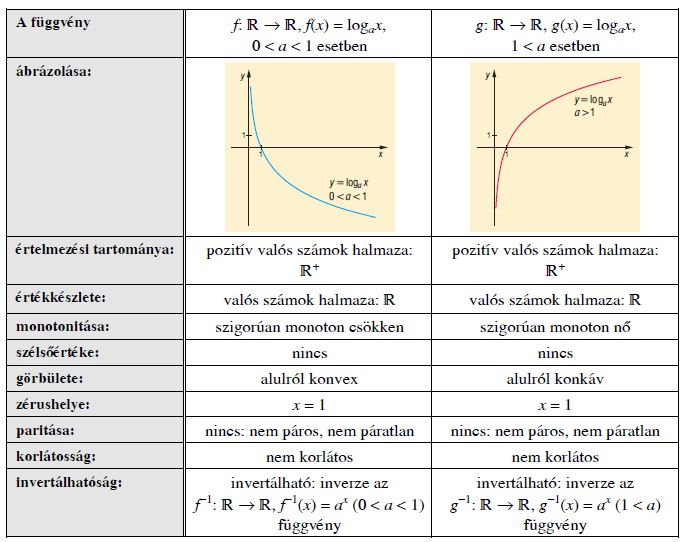
\includegraphics[width=\linewidth]{LogFv.JPG}
	\end{figure}
	Folytonos, differenciálható, integrálható
\section{Alkalmazások}
	\begin{itemize}
		\item Exponenciális egyenletek megoldása
		\item A levegő szerűsége a magassággal exponenciálisan csökken
		\item A Richter-skála logaritmus alapú
		\item Exponenciális függvény írja le a radioaktív izotópok bomlását
	\end{itemize}
\chapter{Egyenlet-megoldási módszerek}
\section{Egyenlet}
	\begin{definition}
		Az egyenlet bármely két egyenlőségjellel összekötött kifejezés. A kifejezésben szereplő
		változók az ismeretlenek.
	\end{definition}
	\begin{definition}
		Az alaphalmaz az ismeretlenek azon értékeinek halmaza, ahol az egyenletet vizsgáljuk,
		ahol a megoldásokat keressük.
	\end{definition}
	\begin{definition}
		Az egyenlet értelmezési tartománya az alaphalmaznak az a legbővebb részhalmaza,
		ahol az egyenletben szereplő kifejezések értelmezhetőek.
	\end{definition}
	\begin{definition}
		Az egyenletet igazzá tevő értékek az egyenlet megoldásai vagy gyökei.
	\end{definition}
	\begin{definition}
		Az alaphalmaz azon elemeinek halmaza, amelyekre az egyenlet igaz, az egyenlet megoldáshalmaza.
	\end{definition}
	\begin{definition}
		Az azonosság olyan egyenlet, amelynek a megoldáshalmaza megegyezik az egyenlet
		értelmezési tartományával.
	\end{definition}
\pagebreak
\section{Egyenlet-megoldási módszerek}
	\begin{outline}[enumerate]
		\1 Mérlegelv
			\2 Két oldal egyforma változtatása
			\2 Megoldáshalmaz nem változik, ha
				\3 az egyenlet mindkét oldalához ugyanazt a számot hozzáadjuk, vagy mindkét oldalából kivonjuk
				\3 az egyenlet mindkét oldalát ugyanazzal a 0-tól különböző számmal szorozzuk, osztjuk
		\1 Grafikus megoldás
			\2 Két oldal ábrázolása
			\2 Közös pont abszcisszája: megoldás
			\2 Hátrány: leolvasás pontatlan lehet
		\1 Szorzattá alakítás
			\2 Egyik oldal->szorzat
			\2 Másik oldal: 0
			\2 Szorzat=0<=>Valamelyik tényező=0
			\2 Pl.:$(x-2)x^2-(x-2)*x=0\implies(x-2)*2x=0$
		\1 Értelmezési tartomány vizsgálata
			\2 Ha $|D|=1$
				\3 Elem ellenőrzése
			\2 Ha $D=0$
				\3 Nincs megoldás
			\2 Pl.: $\sqrt{x-1}-\sqrt{1-x}=0$
				\3 $D={1}$
				\3 1 valóban megoldás
		\1 Értékkészlet vizsgálata
			\2 Két oldal értékkészletének metszetéből kerülhetnek ki a gyökök
			\2 Pl.:	$\frac{16}{3}x^4+\frac{1}{6x^2}=\sin(\pi x)$
				\3 $x\ne0$
				\3 Baloldal: deriválás
					\4 Minimum: $\pm\frac{1}{2}$-nél 1
				\3 Jobboldal: $\le1$
				\3 Bal és jobboldal = 1
				\3 Baloldal=$\pm\frac{1}{2}$
				\3 Jobboldalba helyettesítve csak a pozitív jó
		\1 Új ismeretlen bevezetése
			\2 Pl.: tg$^4(x)-5$tg$^2(x)+4=0\implies a^2-5a+4=0$
	\end{outline}
\section{Ekvivalencia}
	\begin{definition}
		Két egyenlet ekvivalens, ha alaphalmazuk és megoldáshalmazuk is azonos
	\end{definition}
	\begin{definition}
		Ekvivalens átalakítás olyan átalakítás, amit egyenletek megoldása közben végzünk, és az eredetivel ekvivalens egyenletet kapunk.
	\end{definition}
	\begin{outline}
		\1 Ekvivalens: mérlegelv
		\1 Nem ekvivalens: Négyzetre emelés
			\2 Szűkebb értelmezési tartomány: gyökvesztés lehet
			\2 Tágabb értelmezési tartomány: gyöknyerés lehet
	\end{outline}
\section{Gyökvesztés}
	Ismeretlent tartalmazó kifejezéssel való osztás. Például:
	\begin{align*}
		x^3+2x^2+x&=0\tag{Osztás nullával}\\
		x^2+2x+1&=0\\
		x=-1
	\end{align*}
	Helyesen:
	\begin{align*}
		x^3+2x^2+x&=0\\
		x*(x^2+2x)&=0\\
		x&=0\text{, vagy }\\
		x^2+2x=0&\implies x=-1
	\end{align*}
\section{Hamis gyök}
	Négyzetre emelés, például:
	\begin{align*}
		\sqrt{7-x}&=1-x\tag{Négyzetre emelés}\\
		7-x&=x^2-2x+1\\
		x=3&\vee x=-2
	\end{align*}
	Az $x=3$ nem megoldása az eredeti egyenletnek. Kiküszöbölhető közbülső feltétellel: $1-x\ge0$.
\section{Másodfokú egyismeretlenes egyenlet}
	\begin{definition}
		Másodfokú egyismeretlenes egyenlet $ax^2+bx+c=0$ alakra hozható, ahol $a,b,c\in\mathbb{R}$
	\end{definition}
	\begin{theorem}
		$ax^2+bx+c=0$ gyökei: $x_{1,2}=\frac{-b\pm\sqrt{b^2-4ac}}{2a}$, ahol $b^2-4ac\ge0$
	\end{theorem}
	\begin{proof}
		\begin{align*}
			ax^2+bx+c&=0\tag{$*4a$}\\
			4a^2x^2+4abx+4ac&=0\tag{Teljes négyzetté alakítás}\\
			(2ax+b)^2-b^2+4ac&=0\tag{$+b^2-4ac$}\\
			(2ax+b)^2&=b^2-4ac
		\end{align*}
		Mivel a baloldalon négyzetszám van, ami nem lehet negatív, $b^2-4ac$ sem lehet az, ha az lenne, a valós számok körében nincs megoldás. Ha $b^2-4ac\ge0$:
		\begin{align*}
			|2ax+b|&=\sqrt{b^2-4ac}\\
			2ax+b&=\pm\sqrt{b^2-4ac}\\
			2ax&=-b\pm\sqrt{b^2-4ac}\\
			x_{1,2}&=\frac{-b\pm\sqrt{b^2-4ac}}{2a}
		\end{align*}
	\end{proof}
	\begin{definition}
		Az $ax^2+bx+c=0$ másodfokú egyenlet diszkriminánsa $D=b^2-4ac$
	\end{definition}
	\begin{equation*}
	\text{Gyökök száma}=
	\begin{cases*}
		\text{Két különböző valós gyök}, & \text{ha} D>0\\
		\text{Kétszeres gyök}, &\text{ha} D=0\\
		\text{Nincs valós gyök},&\text{ha} D<0
	\end{cases*}
	\end{equation*}
	\begin{theorem}
		A másodfokú egyenlet $ax^2+bx+c=0$ gyöktényezős alakja, ha a diszkrimináns nemnegatív, és a két gyök $x_1$, $x_2$:
		\begin{equation*}
			a*(x-x_1)*(x-x_2)=0
		\end{equation*}
	\end{theorem}
	\begin{theorem}[Vi\`ete-formulák]
		$ax^2+bx+c$ alakú másodfokú egyenlet gyökei, és együtthatói közti összefüggések:
		\begin{align*}
			x_1+x_2&=-\frac{b}{a}\\
			x_1*x_2&=\frac{c}{a}
		\end{align*}
	\end{theorem}
\section{Alkalmazások}
	\begin{itemize}
		\item Egyenes, kör, parabola adott abszcisszájú vagy ordinátájú pontjának meghatározása
		\item Koszinusztételből oldalak kiszámítása
		\item Mély szakadék mélységének meghatározása: egy ledobott kő dobásától a szakadék alján történő koppanás hangjának meghallásáig eltelt idő mérésével.
	\end{itemize}
\chapter{Statisztika}
\section{Adatsokaságok jellemzői}
	A statisztika feladatai közé tartozik, hogy bizonyos egyedek meghatározott tulajdonságairól
	tájékozódjék, majd a szerzett (általában számszerű) adatokat feldolgozza, elemzi.
	\begin{definition}
		Az	elemzéshez összegyűjtött adatok halmazát adatsokaságnak, mintának, a meghatározott tulajdonságot ismérvnek, változónak nevezzük.
	\end{definition}
	\begin{definition}
		A sokaság elemeinek az ismérv szerinti tulajdonságát statisztikai adatnak, az adatsokaság elemeinek számát a sokaság méretének nevezzük.
	\end{definition}
\section{A leíró statisztika jellemzői}
	\begin{outline}
		\1 Tömegesen előforduló jelenségek(ből nyert adatok) vizsgálata
		\1 Adatok összegyűjtése
			\2 Ha vizsgálandó egyedek száma nagy
			\2 Adatsokaság részhalmazát vizsgáljuk
				\3 Mintavétel
				\3 Mintából következtetés a sokaságra
			\2 Reprezentatív mintavétel:
				\3 Tulajdonság előfordulása mintában közelíti a sokaságban való előfordulást
			\2 Véletlenszerű mintavétel:
				\3 Minden elem ugyanakkora valószínűséggel->minta
	\end{outline}
	\begin{definition}
		Az egyes adatok előfordulásának a száma a gyakoriság.
	\end{definition}
	\begin{definition}[Relatív gyakoriság]
		A gyakoriság osztva az adatok számával
	\end{definition}
	\begin{outline}
		\1 Adatok megadása: lehet táblázat
			\2 Nagyobb adathalmazok tömör ábrázolása
			\2 Gyakorisági táblázat: Lehetséges adatok, hozzá tartozó gyakoriságok
		\1 Osztályok
			\2 Nagy méretű adatsokaság, vagy sok különböző érték közel azonos gyakorisággal
			\2 Egymáshoz közeli értékek összevonása
			\2 Diszjunktak, hézagmentesek
	\end{outline}
\section{Diagramok}
	\begin{outline}
		\1 Adatok grafikus megjelenítése
		\1 Oszlopdiagram:
			\2 Adatok egymáshoz való viszonya
			\2 Nem célszerű, ha
				\3 Van 1-2 kiugró érték
				\3 Adatok közötti eltérés nagyon kicsi
			\2 Víszintes tengely: adatfajtáknak megfelelő intervallumok
				\3 Ezek fölé téglalapok
				\3 Területük arányos gyakorisággal
		\1 Hisztogram
			\2 Gyakorisági eloszlás oszlopdiagramon
			\2 Oszlopok hézagmentesen
		\1 Sávdiagram
			\2 Fordított oszlopdiagram
		\1 Kördiagram
			\2 Részadatok egészhez való viszonya
			\2 Alkalmas \%-os adatok ábrázolására
				\3 360\degree: 100\%
			\2 Nem célszerű, ha sok az adat
		\1 Vonaldiagram
			\2 Koordináta-rendszerben pontként
			\2 Töröttvonal köti össze
			\2 Időbeli változás
			\2 Gyakoriságok vonaldiagramja: gyakorisági poligon.
	\end{outline}
\section{Statisztikai mutatók}
	\subsection{Középértékek}
	\begin{outline}
		\1 Adatsokaságokat csak leegyszerűsítve lehet jellemezni
			\2 Középértékek: egy számmal írnak le egy adathalmazt
			\2 Előny: valamilyen tulajdonság jó megjelenítése
			\2 Hátrány: nem nyújtanak képet egyes adatokról
	\end{outline}
\pagebreak
	\begin{outline}
		\1[] \begin{definition}[Módusz]
				Egy adatsokaságban a leggyakrabban előforduló adat.
			\end{definition}
			\2 Ha 1 db van: egymóduszú adatsokaság
				\3 Különben többmóduszú
			\2 Előny: Könnyű meghatározni
			\2 Hátrány: Csak akkor használható jellemzés, ha a többi adathoz képest sokszor fordul elő
		\1[] \begin{definition}[Átlag (számtani közép)]
				Az adatok összegének és az adatok számának hányadosa
			\end{definition}
			\2 $\sum$Nagyobb adatoktól vett eltérések$=\sum$Kisebb adatoktól vett eltérések
			\2 Hátrány: egy kiugró adat eltorzíthatja
		\1[] \begin{definition}[Medián]
			Páratlan számú adat esetén nagyság szerinti sorrendben a középső adat. Páros számú adat esetén a két középső adat átlaga
		\end{definition}
			\2 Összes adat fele $\le$ Medián
			\2 Összes adat fele $\ge$ Medián
			\2 Adatoktól mért távolságok összege minimális
			\2 Előny: valóban középérték
				\3 Ugyanannyi adat nagyobb, mint amennyi kisebb
	\end{outline}
	\subsection{Szóródás jellemzői}
	\begin{outline}
		\1[] \begin{definition}[Terjedelem]
				Legnagyobb és legkisebb adat különbsége
			\end{definition}
			\2 Minél kisebb, annál jobban jellemzi a mintát
		\1[] \begin{definition}[Variancia (szórásnégyzet)]
				Adatok átlagtól való eltérések négyzetének átlaga
			\end{definition}
		\1[] \begin{definition}[Szórás]
				Szórásnégyzet négyzetgyöke:
				\begin{equation*}
					\sigma=\sqrt{\frac{\sum_{i=1}^{n}\left(x_i-\overline{x}\right)^2}{n}}
				\end{equation*}
			\end{definition}
			\2 Megmutatja, adatok mennyire térnek el az átlagtól
			\2 Minél kisebb, átlag annál jobban jellemez
	\end{outline}
\section{Pozitív számok nevezetes közepei}
	\begin{definition}
		$a_1,a_2,\dots,a_n$ nemnegatív számok
		\begin{itemize}
			\item Aritmetikai (számtani) közepe: 
			\begin{equation*}
				A=\frac{\sum_{i=1}^n a_i}{n}
			\end{equation*}
			\item Geometriai (mértani) közepe:
			\begin{equation*}
				G=\sqrt[n]{\prod_{i=1}^n a_i}
			\end{equation*}
			\item Kvadratikus (négyzetes) közepe:
			\begin{equation*}
				Q=\sqrt{\frac{\sum_{i=1}^na_i^2}{n}}
			\end{equation*}
			\item Harmonikus közepe:
			\begin{equation*}
				H=\frac{n}{\sum_{i=1}\frac{1}{a_i}},\text{ ha } a_i>0
			\end{equation*}
		\end{itemize}
	\end{definition}
	\begin{theorem}[Közepek közötti összefüggés]
		\begin{equation*}
		H\le G\le A\le Q
		\end{equation*}
		Egyenlőség csak akkor áll fenn, ha $\forall i,j\ a_i=a_j$
	\end{theorem}
	\begin{theorem}
		Két nemnegatív valós szám esetén $\sqrt{a*b}\le \frac{a+b}{2}$
	\end{theorem}
	\begin{proof}
		Mivel az egyenlőtlenség mindkét oldala nemnegatív, a négyzetre emelés ekvivalens átalakítás.
		\begin{gather*}
			\sqrt{ab}\le\frac{a+b}{2}\Leftrightarrow ab\le\frac{a^2+2ab+b^2}{4}\Leftrightarrow 
			4ab\le a^2+2ab+b^2\Leftrightarrow 0\le a^2-2ab+b^2\Leftrightarrow\\
			\Leftrightarrow 0\le (a-b)^2
		\end{gather*}
		Az utolsó egyenlőtlenség igaz, és mivel mindig ekvivalens átalakításokat végeztünk, az eredeti is igaz.
	\end{proof}
\section{Nevezetes közepek alkalmazása szélsőérték-feladatokban}
	\subsection{Összeg állandósága esetén szorzat maximalizálása.}
	Azon téglatestek közül, amelyek éleinek összege 60 cm, melyiknek a térfogata maximális?
	
	Legyenek a téglatest élei: $a,\ b$ és $c$. Ekkor a térfogata: $V=a*b*c$, az élek összege: $4*(a+b+c)=60$. Ebből $a+b+c=15$. A számtani és mértani közép közötti egyenlőtlenségből:
	\begin{gather*}
		\frac{a+b+c}{3}\ge\sqrt[3]{abc}\implies \left(\frac{a+b+c}{3}\right)^3\ge abc\implies \left(\frac{15}{3}\right)^3\ge abc\implies 5^3\ge abc\implies\\
		\implies 125\ge V
	\end{gather*}
	Mivel egyenlőség csak $a=b=c$ esetén teljesül, így a térfogat az 5 cm élű kocka esetén maximális.
	\subsection{Szorzat állandósága esetén összeg minimalizálása}
	Azon téglalapok közül, amelyeknek a területe $100 cm^2$, melyiknek a kerülete minimális?
	Legyenek a téglalap oldalai $a$ és $b$. Ekkor a területe: $T=ab=100$, kerülete: \\
	$K=2(a+b)$, amiből $\frac{K}{4}=\frac{a+b}{2}$. A számtani és mértani közép közti egyenlőtlenséget kihasználva:
	\begin{equation*}
		\frac{a+b}{2}\ge\sqrt{ab}\implies\frac{K}{4}\ge\sqrt{100}\implies\frac{K}{4}\ge 100\implies K\ge 40
	\end{equation*}
	Mivel egyenlőség csak $a=b$ esetén teljesül, így kerület a 10 cm oldalú négyzet esetén minimális.
\section{Alkalmazások}
	\begin{outline}
		\1 Statisztika
			\2 Közvélemény-kutatások
			\2 Gazdasági mutatók
		\1 Nevezetes közepek
			\2 Négyzetes közép: statisztikai szórás kiszámítása
			\2 Harmonikus közép: átlagsebesség meghatározása
	\end{outline}
\chapter{Számsorozatok}
\section{Számsorozat}
	\begin{definition}
		A számsorozat olyan függvény, amelynek értelmezési tartománya a pozitív egész számok
		halmaza, értékkészlete pedig valamilyen számhalmaz. Az $a_1,\dots,\ a_n$ tagokból álló sorozatot \{$a_n$\}-nel vagy ($a_n$)-nel jelöljük. A sorozat n-edik tagja: $a_n$.
	\end{definition}
	\begin{outline}
		\1 Megadásuk
			\2 Függvényszerűen: $f:\mathbb{N}^+\longrightarrow\mathbb{R},\ x\mapsto x^2$
			\2 Az n-edik általános tagot előállító formulával: $\{a_n\}=3*2^n$
			\2 Az elemeit egyértelműen meghatározó utasítással: $\{a_n\}=\{2^n \text{ utolsó számjegye}\}$
			\2 A sorozat tagjaival: $3,\ 6,\ 9,\dots$
			\2 Rekurzívan: $a_1=1,\ a_2=2,\ a_n=a_{n-1}+a_{n-2},$ ha $n\ge3$
	\end{outline}
\section{Sorozatok tulajdonságai}
	\begin{definition}
		Az $\{a_n\}$ sorozat szigorúan monoton növekvő, ha $\forall n\in\mathbb{Z}^+\ a_n<a_{n+1}$.
	\end{definition}
	\begin{definition}
		Az $\{a_n\}$ sorozat szigorúan monoton csökkenő, ha $\forall n\in\mathbb{Z}^+\ a_n>a_{n+1}$.
	\end{definition}
	\begin{outline}
		\1 Ha csak monotonitás: megengedett egyenlőség is
		\1 Keresése:
			\2 $a_{n+1}-a_n$
			\2 $\frac{a_{n+1}}{a_n}$
				\3 Minden tag pozitív
	\end{outline}
	\begin{definition}
		Egy $\{a_n\}$ sorozatnak $K$ felső korlátja, ha $\forall n\in\mathbb{N}^+\ a_n\le K$. Ilyenkor a sorozatot felülről korlátosnak nevezzük.
	\end{definition}
	\begin{definition}
		Egy $\{a_n\}$ sorozatnak $k$ alsó korlátja, ha $\forall n\in\mathbb{N}^+\ a_n\ge k$. Ilyenkor a sorozatot alulról korlátosnak nevezzük.
	\end{definition}
	\begin{definition}
		Egy sorozat korlátos, ha alulról és felülről is korlátos.
	\end{definition}
	\begin{definition}
		Felülről korlátos sorozat legkisebb felső korlátját a sorozat felső határának (szuprémum, $\sup$), alulról korlátos sorozat legnagyobb alsó korlátját a sorozat alsó határának nevezzük (infimum, $\inf$).
	\end{definition}
	\begin{theorem}
		A valós számok körében felülről korlátos sorozatnak van felső határa, alulról korlátos sorozatnak van alsó határa.
	\end{theorem}
	\begin{theorem}
		Végtelen sok egymásba skatulyázott, zárt intervallumnak a valós számok körében van közös pontja. Ha az intervallumok hossza minden pozitív számnál kisebbé válik, akkor pontosan egy közös pont van.
	\end{theorem}
	\begin{definition}
		Az \{$a_n$\} sorozat konvergens és határértéke az $A$ szám, ha
		\begin{equation*}
			\forall\epsilon>0\ \exists N\in\mathbb{Z}^+\ n>N\implies|a_n-A|<\epsilon
		\end{equation*}
		Jelölése: $\lim\limits_{n\rightarrow\infty}a_n=A$, vagy $a_n\rightarrow A$.
	\end{definition}
	\begin{definition}
		Az olyan sorozatokat, amelyeknek nincs határértéke, divergens sorozatoknak nevezzük.
	\end{definition}
	\begin{theorem}[]
		Konvergens sorozatok tulajdonságai:
		\begin{itemize}
			\item Csak egy határértéke van
			\item Korlátos
			\item Ha monoton és korlátos, akkor konvergens. Határérték növekedés esetén felső, csökkenés esetén alsó határ
			\item Rendőr-elv: $\left(\left(\left(\forall n\in\mathbb{N}^+\ a_n\le b_n\le c_n\right)\wedge a_n\rightarrow A\right)\wedge c_n\rightarrow A\right)\implies b_n\rightarrow A$
		\end{itemize}
	\end{theorem}
\section{Műveletek konvergens sorozatokkal}
	\begin{outline}
		\1 $\{a_n\},\ \{b_n\}$ konvergens, és $a_n\rightarrow A, b_n\rightarrow B$
			\2 $a_n\pm b_n\rightarrow A\pm B$
			\2 $a_n*b_n\rightarrow A*B$
			\2 $c*a_n\rightarrow c*A$, ahol $c\in\mathbb{R}$
			\2 $\frac{a_n}{b_n}\rightarrow\frac{A}{B}$, ahol $b_n\ne0,\ B\ne0$
	\end{outline}
\section{Számtani sorozat}
	\begin{definition}
		Azt a számsorozatot, amelyben a második tagtól kezdve bármely tag és a közvetlenül
		előtte álló tag különbsége állandó, számtani sorozatnak nevezzük. Ez a különbség a differencia, jele $d$.
		\begin{equation*}
		\begin{cases*}
			\text{Szigorúan monoton nő, és alulról korlátos ha} & d>0\\
			\text{Konstans, ha} & d=0\\
			\text{Szigorúan monoton csökken, és felülről korlátos, ha} & d<0
		\end{cases*}
		\end{equation*}
	\end{definition}
	\begin{theorem}
		Ha egy számtani sorozat első tagja $a_1$, differenciája $d$, akkor n-edik tagja $a_n=a_1+(n-1)*d$.
	\end{theorem}
	\begin{theorem}
		A számtani sorozat első n tagjának összege ($S_n$) az első és az n-edik tag számtani közepének n-szeresével egyenlő: $S_n=\frac{a_1+a_n}{2}*n$
	\end{theorem}
	\begin{proof}
		Az összeget felírjuk az 1., majd az n-edik tagtól kiindulva:
		\begin{align*}
			S_n&=\sum_{i=1}^{n} a_n=\sum_{i=1}^n (a_1+(i-1)*d)\\
			S_n&=\sum_{i=1}^n a_{n-i+1}=\sum_{i=1}^{n} (a_n-(i-1)*d)\\
		\end{align*}
		A kettőt összeadva:
		\begin{align*}
			2S_n&=\sum_{i=1}^{n} (a_1+a_n)=n*(a_1+a_n)\\
			S_n&=\frac{a_1+a_n}{2}*n\qedhere
		\end{align*}
	\end{proof}
	\begin{theorem}
		$S_n$ másik alakja:
		\begin{equation*}
			S_n=\frac{2a_1+(n-1)d}{2}*n
		\end{equation*}
	\end{theorem}
	\begin{theorem}
		Tetszőleges elem a tőle szimmetrikusan elhelyezkedőknek a számtani közepe:
		\begin{equation*}
			a_n=\frac{a_{n-k}+a_{n+k}}{2}
		\end{equation*}
	\end{theorem}
\section{Alkalmazások}
	\begin{itemize}
		\item Irracionális kitevőjű hatvány fogalma sorozat határértékével.
		\item Speciális függvények közelítése polinomokkal, pl.:
		\begin{align*}
			\sin(x)&=x-\frac{x^3}{3!}+\frac{x^5}{5!}-\dots=\sum_{n=0}^{\infty} \left(\frac{(-1)^n*x^{2n-1}}{(2n-1)!}\right)\\
			\cos(x)&=1-\frac{x^2}{2!}+\frac{x^4}{4!}-\dots=\sum_{n=0}^{\infty} \left(\frac{(-1)^n*x^{2n}}{(2n)!}\right)\\
		\end{align*}
		\item Analízis: függvény határértékénél, folytonosságánál
	\end{itemize}
\chapter{Mértani sorozat}
\section{Mértani sorozat}
	\begin{definition}
		A számsorozat olyan függvény, amelynek értelmezési tartománya a pozitív egész számok
		halmaza, értékkészlete pedig valamilyen számhalmaz. Az $a_1,\dots,\ a_n$ tagokból álló sorozatot \{$a_n$\}-nel vagy ($a_n$)-nel jelöljük. A sorozat n-edik tagja: $a_n$.
	\end{definition}
	\begin{definition}
		Azt a számsorozatot, amelyben a második tagtól kezdve bármely tag és a közvetlenül
		előtte álló tag hányadosa állandó, mértani sorozatnak nevezzük. Ez a hányados a kvóciens,
		jele $q$. A definíció kizárja, hogy a sorozat bármely eleme 0 legyen, továbbá a kvóciens sem lehet 0.
	\end{definition}
	\begin{theorem}
		Ha egy mértani sorozat első tagja $a_1$, hányadosa $q$, akkor n-edik tagja $a_n=a_1*q^{n-1}$
	\end{theorem}
	\begin{theorem}
		A mértani sorozat első n tagjának összege:
			\begin{equation*}
			S_n=
			\begin{cases*}
			n*a_1,& ha $q=1$\\
			a_1*\frac{q^n-1}{q-1},& ha $q\neq 1$
			\end{cases*}
		\end{equation*}
	\end{theorem}
	\begin{proof}
		Ha $q=1$, akkor a sorozat minden tagja $a_1$, így: $S_n=\sum_{i=1}^{n} a_1=n*a_1$. Ha $q\ne1$, akkor:
		\begin{align*}
			S_n&=\sum_{i=1}^n a_1*q^{i-1}\\
			q*S_n&=\sum_{i=1}^n a_1*q^i\\
			S_n*q-S_n&=a_1*q^n-a_1\tag{Két egyenletet kivonva egymásból}\\
			S_n(q-1&=a_1*(q^n-1)\\
			S_n&=a_1*\frac{q^n-1}{q-1}\tag{Mindkét oldal osztva $q-1\ne0$-val}
		\end{align*}
	\end{proof}
	\begin{theorem}
		Bármely elem négyzete egyenlő a tőle szimmetrikusan elhelyezkedő tagok szorzatával:
		\begin{equation*}
			a_n^2=a_{n-k}*a_{n+k}
		\end{equation*}
	\end{theorem}
	\begin{theorem}
		Pozitív tagú sorozatnál bármely elem a tőle szimmetrikusan elhelyezkedő elemek mértani
		közepe:
		\begin{equation*}
			a_n=\sqrt{a_{n-k}*a_{n+k}}\text{, ha }\forall n\in\mathbb{N}^+\ a_n>0
		\end{equation*}
	\end{theorem}
	\begin{theorem}[Mértani sorozat konvergenciája]
		\begin{equation*}
			\begin{cases*}
				a_n\longrightarrow a_1,& ha $q=1$\\
				a_n\longrightarrow 0,& ha $|q|<1$\\
				\{a_n\}\text{ divergens},& ha $q=-1\vee|q|>1$
			\end{cases*}
		\end{equation*}
	\end{theorem}
\section{Végtelen mértani sor}
	\begin{definition}
		Legyen $\{a_n\}$ egy számsorozat A $\sum_{i=1}^\infty a_i$ összeget végtelen sornak nevezzük.
	\end{definition}
	\begin{definition}
		Ha a $\sum_{i=1}^\infty a_i$ végtelen sorban \{$a_i$\} sorozat egy mértani sorozat, akkor a végtelen sort mértani sornak nevezzük.
	\end{definition}
	\begin{definition}
		A sor összegén a $\lim\limits_{n\to\infty} S_n=\lim\limits_{n\to\infty} \sum_{i=1}^n a_i$ határértéket értjük, amennyiben létezik.
	\end{definition}
	\begin{theorem}
		Ha egy mértani sorban $|q|<1$, akkor a mértani sor konvergens, és összege $S=\frac{a_1}{1-q}$, ha $|q|\ge1$, akkor nem konvergens.
	\end{theorem}
\section{Kamatszámítás}
	\begin{outline}
		\1 Kamat: tőke használatáért járó díj
			\2 Tőke: Kölcsönadott, letétbe helyezett pénz
			\2 Nagysága: tőke százalékában (kamatláb)
			\2 Kamattényező: 
				\3 Értéknövekedés: $q=1+\frac{p}{100}$
				\3 Értékcsökkenés: $q=1-\frac{p}{100}$
		\1 Kamatos kamat: Kamatozás után, kamat+tőke kamatozik
			\2 Mértani sorozat
				\3 Van nulladik tag (a)
			\2 $a$ összeg $p\%$-ot kamatozik évente, akkor az $n$-edik év végére az összeg:\\ $a_n=a*\left(1+\frac{p}{100}\right)^n$
			\2 Éves kamatláb $p\%$, akkor
				\3 Havi: $\sqrt[12]{1+\frac{p}{100}}$
				\3 Napi: $\sqrt[365]{1+\frac{p}{100}}$
	\end{outline}
\section{Gyűjtőjáradék}
	\begin{outline}
		\1 Alapösszeget időközönként azonos összeggel növelünk, a teljes összeg kamatozik
		\1 Minden év elején $a$ összeget teszünk be, ez $p\%$-al kamatozik.
			\2 $q=1+\frac{p}{100}$
			\2 n-edik év végén: mértani sorozat első n elemének összege, ahol $a_1=aq$. $S_n=a*q\frac{q^n-1}{q-1}$
	\end{outline}
\section{Törlesztőrészlet}
	\begin{outline}
		\1 Hitelt egyenlő időközönként ugyanakkora összeggel fizetünk vissza, mindig a fennálló tartozásra fizetjük a kamatos kamatot
		\1 $n$ évre $S_n$ nagyságú hitelt évi $p\%$-os kamatra veszünk fel, minden évben $a$ összeget törlesztünk.
			\2 $n$-edik év végén befizetések kamatokkal megnövelt értéke egyenlő a kölcsön $n$ év alatt $p\%$-os kamatozással megnőtt értékével. Ha $q=1+\frac{p}{100}$, akkor $S_n*q^n=a*\frac{q^n-1}{q-1}$.
	\end{outline}
\section{Exponenciális folyamatok}
	\begin{outline}
		\1 Időben növekedés: $N_t=N_0*e^{\lambda t}$, csökkenés: $N_t=N_0*e^{-\lambda t}$.
			\2 $N_0$ - kezdeti mennyiség, $N_t$ - t időpontbeli mennyiség, $\lambda$ - folyamatra jellemző paraméter
		\1 Minél nagyobbak, annál gyorsabban növekednek. Változást exponenciális függvény írja le.
		\1 Föld túlnépesedése
			\2 Matematikai modell: 1837 óta minden évben 1,1\%-al nő: $N_t=1*1,011^t$.
				\3 Kb. 63 évente duplázódik
			\2 Ugyanannyi időközönként egyre nagyobb számmal nő népesség
			\2 Rendelkezésre álló erőforrások nem tudnak lépést tartani
			\2 Vagy életfeltételek romlása, vagy népesség növekedése csökken
		\1 Diszkrét exponenciális növekedés: kamatos kamat
		\1 Diszkrét exponenciális csökkenés: tárgyak értékcsökkenése
			\2 Évi $p\%$-os: $a_n=a*\left(1-\frac{p}{100}\right)^n$
		\1 Térbeli: sugárzások elnyelődése homogén közegben
	\end{outline}
\section{Alkalmazások}
	\begin{outline}
		\1 Végtelen szakaszos tizedestörtek közönséges tört alakra hozása: konvergens mértani sor tulajdonságai
		\1 Exponenciális függvény:
			\2 Radioaktív izotópok bomlási egyenletei
			\2 Oldódás folyamata
			\2 Kondenzátor feltöltődésének, kisülésének folyamata
	\end{outline}
\chapter{Deriválás}
\section{Függvény fogalma, értelmezési tartomány, értékkészlet}
	
\end{document}